\chapter{Resultados e discussão}\label{Resultados}

\section{Efeito do \textit{setup} das simulações}\label{EfeitoDoSetup}

\subsection{Interações de Lennard-Jones}

A Tabela \ref{tab:Rg} contém os valores dos raios de giro calculados para ambos os \textit{setups} considerados na Seção \ref{ProtocoloDeSimulacao}. 
Nas colunas ``PME'' e ``CUT'' os erros absolutos são da ordem de $0.01$ nm. 
Logo, conclui-se que a mudança do algoritmo para avaliação das interações de Lennard-Jones não afeta o raio de giro.

Claro que diferentes distribuições de partículas podem gerar o mesmo raio de giro para diferentes estruturas.
Mas a análise de funções de distribuição radial também não revelou alterações significativas frente a mudança do algoritmo de avaliação.

Visto isso, somente serão apresentados os resultados obtidos utilizando o método do \textit{cut-off} com raio de corte de $1.2$ nm, que é a configuração ótima obtida pelo trabalho de Gonçalvez \textit{et al}\cite{Goncalvez2018} em um estudo muito mais abrangente e sistemático na avaliação de configurações de simulação utilizando o 2016H66\cite{Horta2016} no GROMACS\cite{VanDerSpoel2005}.
As curvas utilizando o método PME são mostradas nos apêndices \ref{PAMAMap} e \ref{PPIap}.

%\begin{landscape}
\begin{table}[ht!]
\centering
\begin{tabular}{c|ccc|cccc}
\hline
  Environment   & \multicolumn{3}{c|}{PAMAM} & \multicolumn{4}{c}{PPI} \\
\hline
\multirow{2}{*}{pH}    & \multirow{2}{*}{G} &   This work & This work & \multirow{2}{*}{G} & This work & This work & This work  \\
&                               &   (PME)       &   (CUT)   &                               &   (PME)   &   (CUT)  &   (NEWPROT) \\
\hline
\hline
\multirow{6}{*}{Low} & 0    &   0.58  &   0.59  & 1 &  0.51  &   0.51  &   - \\
                        & 1    &   1.01  &   1.00  & 2 &  0.78  &   0.79  &   - \\
                        & 2    &   1.47  &   1.48  & 3 &  1.04  &   1.06  &   - \\
                        & 3    &   1.91  &   1.97  & 4 &  1.34  &   1.35  &   - \\
                        & 4    &   2.45  &   2.46  & 5 &  1.65  &   1.65  &   - \\
                        & 5    &   2.99  &   2.97  & 6 &  1.99  &   2.00  &   - \\
\hline
\multirow{6}{*}{Neutral}& 0 &   0.51  &   0.50  & 1 &  0.51  &   0.49  &   0.51 \\
                        & 1    &   0.79  &   0.79  & 2 &  0.77  &   0.76  &   0.77 \\
                        & 2    &   1.06  &   1.06  & 3 &  1.04  &   1.01  &   1.05 \\
                        & 3    &   1.45  &   1.45  & 4 &  1.34  &   1.30  &   1.33 \\
                        & 4    &   1.84  &   1.99  & 5 &  1.65  &   1.60  &   1.65 \\
                        & 5    &   2.53  &   2.51  & 6 &  1.98  &   1.91  &   1.98 \\
\hline
\multirow{6}{*}{High} & 0   &   0.49  &   0.48  & 1 &  0.49  &   0.49  &   - \\
                        & 1    &   0.75  &   0.72  & 2 &  0.74  &   0.74  &   - \\
                        & 2    &   0.99  &   1.00  & 3 &  0.95  &   0.94  &   - \\
                        & 3    &   1.24  &   1.18  & 4 &  1.07  &   1.03  &   - \\
                        & 4    &   1.60  &   1.56  & 5 &  1.25  &   1.31  &   - \\
                        & 5    &   1.96  &   1.96  & 6 &  1.60  &   1.56  &   - \\
\hline
\end{tabular}
\caption{Raio de giro $R_g$ (nm) obtidos nesse trabalho. Comparação quantitativa entre as diferentes configurações consideradas para as simulações feitas.}
\label{tab:Rg}
\end{table}
%\end{landscape}


\subsection{Protonação do PPI}\label{ProtonacaoPPI}

Como discutido na Seção \ref{SistemasSimulados}, dois estados de protonação distintos foram considerados para tratar o PPI em meio com pH neutro. 
Pela última coluna da Tabela \ref{tab:Rg}, é possível notar que, considerando um grau de protonação maior que o sugerido pelo modelo de Ising\cite{VanDuijvenbode1998, Koper1997}, não há uma alteração significativa do raio de giro quando aminas terciárias no PPI são protonadas.
Essa estrutura foi, também, simulada utilizando ambos os protocolos de avaliação das interações de Lennard-Jones (\textit{cut-off} e PME).
Mas os resultados, assim como os discutidos na seção anterior, não apresentam diferenças significativas.
Por isso, somente os resultados utilizando \textit{cut-off} são apresentados para essa protonação na Tabela \ref{tab:Rg}.

Pela análise das funções de distribuição radial, pode-se notar que a distribuição de aminas primárias sofre uma leve alteração em gerações maiores.
A escolha do PPI de acordo com o modelo de Ising\cite{VanDuijvenbode1998, Koper1997}, leva a uma distribuição onde há uma menor densidade de aminas terminais no interior do dendrímero e, consequentemente, um maior acúmulo na região superficial.
Esse é o comportamento encontrado nas estruturas em meio ácido.
Como consideramos um estado de protonação mais próximo ao que seria quando em pH baixo, o comportamento naturalmente tendeu à uma distribuição em maior acordo com o meio.

Como somente o raio de giro é uma propriedade de validação quantitativa, ambos os modelos de perfis de protonação podem ser considerados adequados.
No entanto, considerando uma avaliação qualitativa da forma das funções de distribuição radial em relação à outros trabalhos computacionais e teóricos o modelo de Ising\cite{VanDuijvenbode1998, Koper1997} parece ser mais adequado. Os resultados mostrados na Seção \ref{PPIEstrutura} são os obtidos de acordo com o modelo de Ising\cite{VanDuijvenbode1998, Koper1997} por serem análises mais refinadas do que a simples suposição de protonação semelhar ao PAMAM.

Os resultados obtidos são apresentados abaixo e foram separados em duas seções: Uma para a discussão do PAMAM e outra para o PPI. Dessa forma, detalhes específicos de cada um dos dendrímeros poderão ser melhor discutidos.

\begin{landscape}
\begin{table*}[t] %PAMAM Rg Suplemmental info tables
\centering
\caption{Comparação do raio de giro $R_g$ (em nm) calculado na presente dissertação para o PAMAM com valores disponíveis na literatura.
Os resultados estão organizados de acordo com o pH do meio (baixo, neutro e alto), número da geração $GN$ (de G0 à G5) e método utilizado no tratamento das interações de Lennard-Jones (PME: Particle-Mesh Ewald e CUT: \textit{cut-off scheme} com raio de corte de $1.2$ nm).
Os resultados da literatura mostrados foram tirados dos seguintes estudos:
SAXS(Prosa1997)\cite{Prosa1997},
SAXS(Rathgeber2002)\cite{Rathgeber2002},
CVFF(Lee2002)\cite{Lee2002},
Dreiding(Maiti2004)\cite{Maiti2004},
Dreiding(Maiti2005)\cite{Maiti2005},
GAFF(Opitz2006)\cite{Opitz2006},
SANS(Porcar2008)\cite{Porcar2008},
GAFF(Maingi2012)\cite{Maingi2012},
CHARMM(Caballero2013)\cite{Caballero2013},
CHARMM and GROMOS(Kanchi2018)\cite{Kanchi2018},
GAFF(Barraza2018)\cite{Barraza2018}.}
\scalebox{0.8}{
\begin{tabular}{cccccccccccccccc}
\hline
G$N$ & \multirow{2}{*}{pH}    & \multicolumn{2}{c}{This work} &GAFF\cite{Maingi2012}&    Dreiding\cite{Maiti2005}  & Dreiding\cite{Opitz2006} &Dreiding\cite{Maiti2004}  & CVFF\cite{Lee2002}     & GAFF\cite{Barraza2018}    &CHARMM\cite{Caballero2013}        &CHARMM\cite{Kanchi2018}   &GROMOS\cite{Kanchi2018}   &     SANS\cite{Porcar2008} & SAXS\cite{Rathgeber2002} & SAXS\cite{Prosa1997}\\
PAMAM   &               &   PME &   CUT &   &  &    &   &   &   &   &   &   &   &   &   \\
%   PAMAM   &               &   PME &   CUT &   Maingi2012      &   Maiti2005               &   Opitz2006           &Maiti2004              &   Lee2002             &   Barraza2018         &   Caballero2013           &Kanchi2018             &Kanchi2018             &   Porcar2008      & Rathgeber2002     & Prosa1997         \\
\hline
\hline
G0    & \multirow{6}{*}{Low} & 0.58  & 0.59          &       -           & -                         &   -                   &-                      &   -                   &   -                   &-                          &-                      &-                      &   -               &   -               &   -\\
G1   &                          & 1.01  & 1.00      &       -           & -                         &   -                   &-                      &   -                   &   -                   &-                          &-                      &-                      &   -               &   -               &   -\\
G2  &                          & 1.47  & 1.48      &       -           & -                         &   1.24                &-                      &   1.66                &   -                   &-                          &-                      &-                      &   -               &   -               &   -\\
G3     &                          & 1.91  & 1.97      &       -           & -                         &   1.64                &-                      &   2.28                &   -                   &-                          &-                      &-                      &   1.704           &   -               &   -\\
G4    &                          & 2.45  & 2.46      &       -           & 1.90                      &   2.13                &-                      &   2.99                &   -                   &-                          &-                      &-                      &   2.158           &   -               &   -\\
G5   &                          & 2.99  & 2.97      &       -           & 2.48                      &   2.65                &-                      &   3.80                &   -                   &-                          &-                      &-                      &   2.6839          &   -               &   -\\
\hline
G0     & \multirow{6}{*}{Neutral} & 0.51  & 0.50      &       -           & -                         &   -                   &-                      &   -                   & 0.61                  &-                          &-                      &-                      &       -           &   0.4             &   -   \\
G1    &                          & 0.79  & 0.79      &       -           & -                         &   -                   &-                      &   -                   & 0.93                  &-                          &-                      &-                      &       -           &   0.79            &   -       \\
G2   &                          & 1.06  & 1.06      &       -           & -                         &   0.95                &-                      &   1.45                & 1.26                  &-                          &-                      &-                      &       -           &   1.18            &   -       \\
G3  &                          & 1.45  & 1.45      &   1.578           & -                         &   1.21                &-                      &   1.97                & 1.52                  &1.533                      &1.408                  &1.619                  &   1.666           &   1.509           &   1.58    \\
G4     &                          & 1.84  & 1.99      &   2.064           & 1.70                      &   1.49                &-                      &   2.67                &   -                   &2.104                      &-                      &-                      &   2.129           &   1.86            &   1.71    \\
G5    &                          & 2.53  & 2.51      &   2.532           & 2.22                      &   2.08                &-                      &   3.28                &   -                   &2.550                      &-                      &-                      &   2.641           &   2.307           &   2.41    \\
\hline
G0   & \multirow{6}{*}{High}    & 0.49  & 0.48      &       -           & -                         &   -                   & 0.493                 &   -                   & 0.58                  &-                          &-                      &-                      &       -           &   -               &   -       \\
G1  &                          & 0.75  & 0.72      &       -           & -                         &   -                   & 0.746                 &   -                   & 0.84                  &-                          &-                      &-                      &       -           &   -               &   -       \\
G2     &                          & 0.99  & 1.00      &       -           & -                         &   0.94                & 0.917                 &   0.84                & 1.01                  &-                          &-                      &-                      &       -           &   -               &   -   \\
G3    &                          & 1.24  & 1.18      &   1.227           & -                         &   1.16                & 1.123                 &   1.16                & 1.31                  &-                          &-                      &-                      &   1.619           &   -               &   -       \\
G4   &                          & 1.60  & 1.56      &   1.550           & 1.68                      &   1.42                & 1.450                 &   1.48                & -                     &-                          &-                      &-                      &   2.092           &   -               &   -   \\
G5  &                          & 1.96  & 1.96      &   1.900           & 2.03                      &   1.80                & 1.834                 &   1.83                & -                     &-                          &-                      &-                      &   2.586           &   -               &   -   \\
\hline
\end{tabular}}
\label{tab:PAMAMRgValidacao}
\end{table*}
\end{landscape}

\section{PAMAM}

\subsection{Tamanho}\label{PAMAMTamanho}
O raio de giro foi calculado de acordo com o descrito na Seção \ref{RaioDeGiro} para cada sistema PAMAM relatado na Seção \ref{SistemasSimulados} e na Tabela \ref{tab:sistemas}, ou seja, das gerações 0 à 5 em meios com pH ácido, neutro e básico.
Os valores mostrados nas curvas a seguir estão listados na Tabela \ref{tab:PAMAMRgValidacao}.
Nela se encontram tanto os raios de giro dos sistemas simulados nesse trabalho quanto os disponíveis na literatura experimental e de simulação utilizados para validação.

\begin{figure}[ht!]
\centering
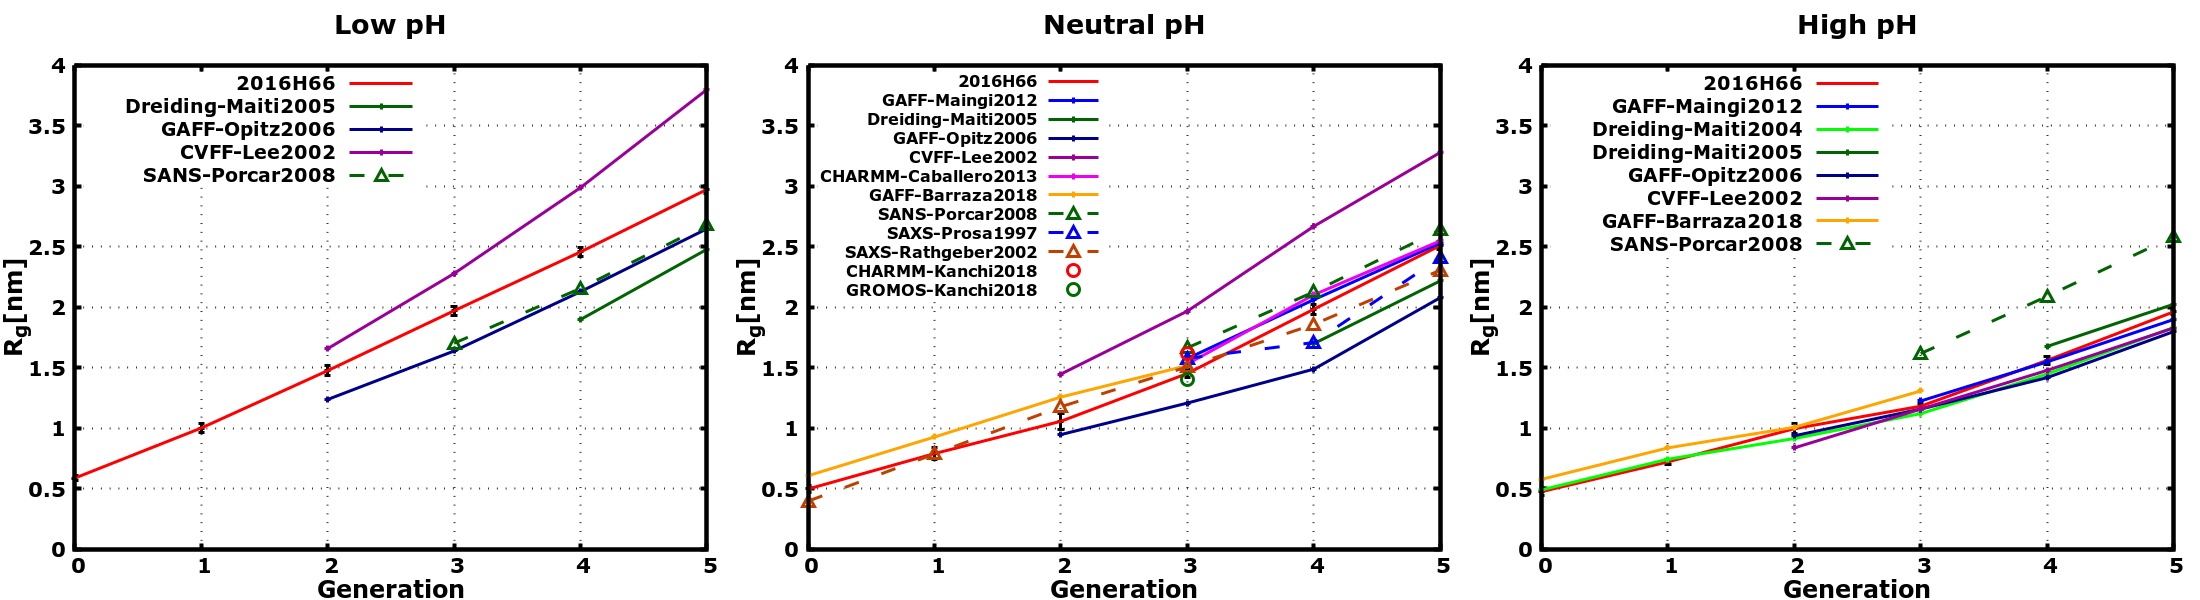
\includegraphics[width=\textwidth]{images/PAMAMRg.png}
\caption{Raio de giro ($R_g$) em função da geração em meios de pH baixo (imagem da esquerda), neutro (imagem do meio) e alto (imagem da direita).
Os resultados obtidos com o campo de força 2016H66\cite{Horta2016} são comparados com resultados de estudos experimentais e de simulações prévios:
Prosa1997\cite{Prosa1997}, %\cite{PR97.2},
Lee2002\cite{Lee2002}, %\cite{LE02.8},
Caballero2013\cite{Caballero2013}, %\cite{CA13.4},
Rathgeber2002\cite{Rathgeber2002}, %\cite{RA02.6},
Maiti2005\cite{Maiti2005}, %\cite{MA05.26},
Opitz2006\cite{Opitz2006}, %\cite{OP06.1},
Porcar2008\cite{Porcar2008}, %\cite{PO08.3},
Maiti2009\cite{Maiti2009}, %\cite{MA09.18},
Maingi2012\cite{Maingi2012}, %\cite{MA12.23},
Barraza2018\cite{Barraza2018}, %\cite{BA18.Y},
Kanchi2018\cite{Kanchi2018}.} %\cite{KA18.Y}.}
\label{fig:PAMAMRg}
\end{figure}


Quando em baixo pH, podemos ver que o 2016H66\cite{Horta2016} mantêm uma tendência quase linear assim como o resultado de espalhamento de neutrons a baixos ângulos (SANS) obtido por Porcar \textit{et al}\cite{Porcar2008}, mesmo que o 2016H66\cite{Horta2016} superestime os resultados consistentemente, em relação ao experimental.
Diferentemente, Lee \textit{et al}\cite{Lee2002} obtiveram um resultado que superestima consideravelmente o raio de giro de forma exponencial com o aumento da geração utilizando o campo de força CVFF\cite{Lifson1979} modelando o solvente implicitamente. 
Maiti \textit{et al}\cite{Maiti2005} conseguiram valores significativamente em acordo com os resultados reportados de SANS\cite{Porcar2008} utilizando o campo de força Dreiding\cite{Mayo1990} com moléculas de água e contra-íons explícitos no sistema.
Curiosamente, os resultados obtidos por Opitz e Wagner\cite{Opitz2006} revelaram um excelente acordo com os dados experimentais da literatura ao simular o PAMAM de gerações 2 a 5 usando metanol como solvente explicitamente. 

Em pH neutro, os resultados obtidos por Lee \textit{et al} continuam a superestimar exponencialmente todos os valores de raio de giro em relação aos estudos reportados na literatura, tanto experimental quanto de simulação.
Enquanto o estudo feito com o campo de força GAFF por Opitz e Wagner\cite{Opitz2006} subestima significativamente todos os outros resultados disponíveis na faixa de gerações estudada nesse trabalho.
O 2016H66\cite{Horta2016} está em excelente acordo com os resultados experimentais de SAXS reportados por Rathgeber \textit{et al}\cite{Rathgeber2002} e subestima um pouco os valores da propriedade quando comparados com o resultado de SANS reportados por Porcar \textit{et al}\cite{Porcar2008}, comportamento inverso do observado em baixo pH.
Os resultados de Prosa \textit{et al}\cite{Prosa1997} desviam fortemente do perfil quase linear apresentado pelos outros estudos disponíveis na literatura. Por isso, não existe um estudo que consistentemente esteja em acordo com os valores reportados por eles.
Podemos ver na imagem central da Figura \ref{fig:PAMAMRg} que em geração 3 os trabalhos com os campos de força CHARMM\cite{Caballero2013, Kanchi2018}, GAFF\cite{Maingi2012, Barraza2018}, 2016H66 (este trabalho) e até mesmo os resultados de SAXS\cite{Rathgeber2002} estão em bom acordo com os estudos de Prosa \textit{et al}\cite{Prosa1997}.
Mas em geração 4, podemos ver que somente o campo de força Dreiding \cite{Maiti2005} apresenta um bom acordo com ele.
Em relação à outros trabalhos de simulação, o 2016H66\cite{Horta2016} está em excelente acordo com os resultados de Maingi \textit{el al}\cite{Maingi2012} e de Caballero \textit{et al}\cite{Caballero2013} para as gerações de 3 à 5 (gerações disponíveis para comparação).
Especialmente para a geração 3, o 2016H66\cite{Horta2016} apresenta um excelente acordo com o valor reportado por Kanchi \textit{et al}\cite{Kanchi2018} para sua simulação utilizando o campo de força GROMOS86, trabalho no qual o autor mostra que esse campo de força foi o único capaz de reproduzir qualitativamente a superfície de energia livre de adsorção do dendrímero em uma membrana lipídica.

Já em alto pH, todos os trabalhos de simulação reportados estão relativamente de acordo, independentemente do campo de força e configurações utilizadas para o sistema.
E todos subestimam o raio de giro quando comparados com os resultados de SANS\cite{Porcar2008} disponíveis.

\begin{figure}[ht!]
\centering
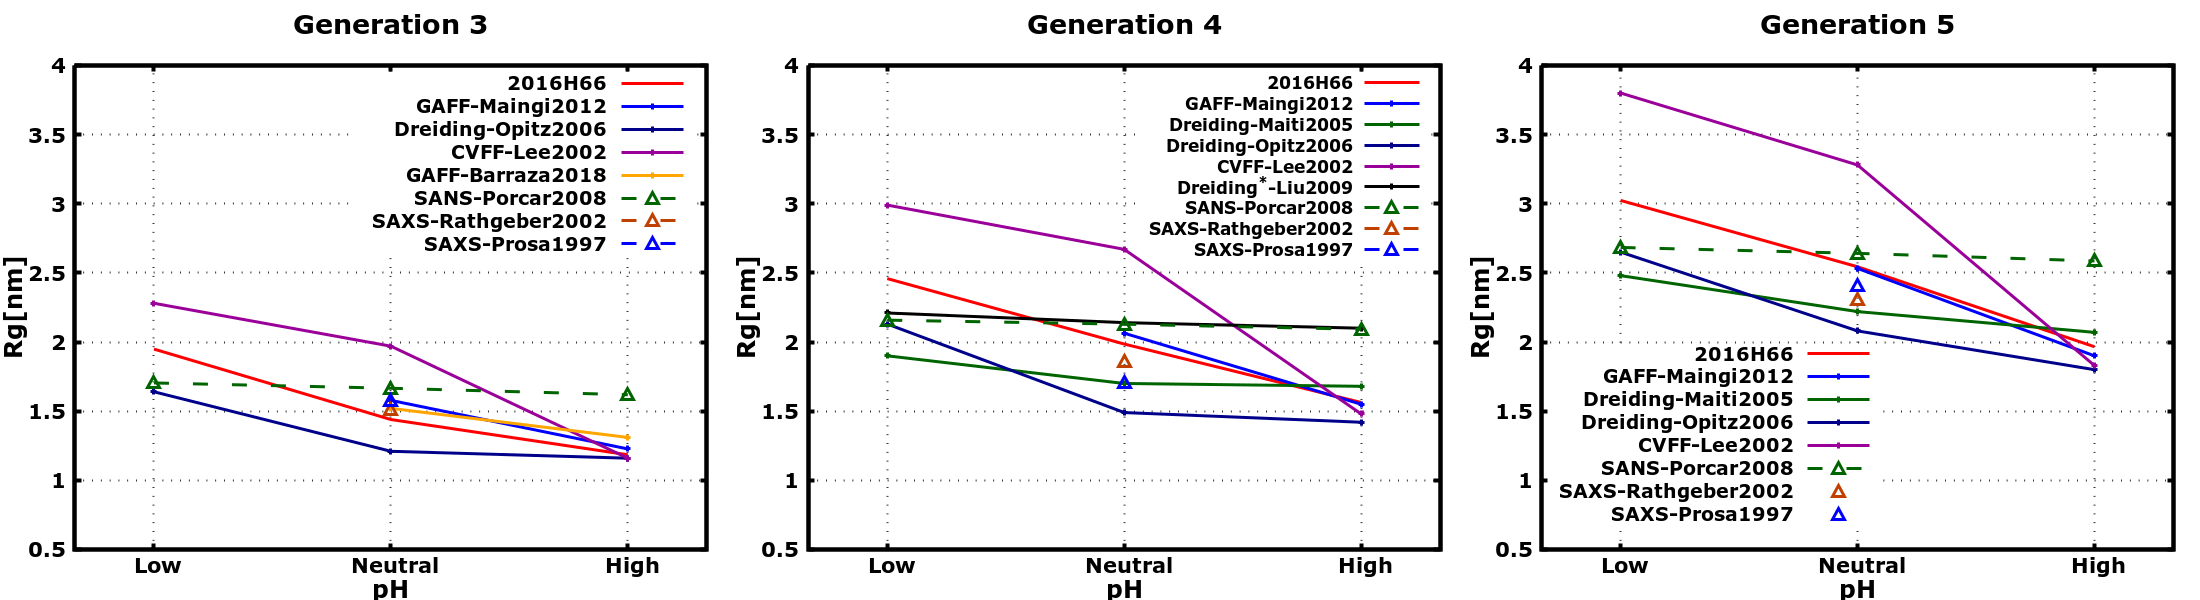
\includegraphics[width=\textwidth]{images/PAMAMgyrateGpH.png}
\caption{Raio de giro ($R_g$) em função do pH para o PAMAM de geração 3 (imagem da esquerda), 4 (imagem do meio) e 5 (imagem da direita).
Os resultados obtidos com o campo de força 2016H66\cite{Horta2016} são comparados com resultados de estudos experimentais e de simulações prévios:
Prosa1997\cite{Prosa1997}, %\cite{PR97.2},
Lee2002\cite{Lee2002}, %\cite{LE02.8},
Rathgeber2002\cite{Rathgeber2002}, %\cite{RA02.6},
Maiti2005\cite{Maiti2005}, %\cite{MA05.26},
Opitz2006\cite{Opitz2006}, %\cite{OP06.1},
Porcar2008\cite{Porcar2008}, %\cite{PO08.3},
Liu2009\cite{Liu2009}, %\cite{LI09.Y},
Maingi2012\cite{Maingi2012}, %\cite{MA12.23}.  }
Barraza2018\cite{Barraza2018}.} %\cite{BA18.Y},
\label{fig:PAMAMRgpH}
\end{figure}

Como foi discutido anteriormente, os valores obtidos com o campo de força 2016H66\cite{Horta2016} superestimam os resultados de SANS de Porcar \textit{et al}\cite{Porcar2008} em pH baixo e começam a subestimá-los em pH neutro e alto.
Esse comportamente se deve ao fato dos valores de SANS serem praticamente invariantes com o pH.
Como pode ser visto mais facilmente na Figura \ref{fig:PAMAMRgpH}, onde foi plotado os valores do raio de giro em função do pH para as gerações de 3 à 5.

A curva referente aos resultados de SANS\cite{Porcar2008} são constantes enquanto nas curvas de simulação os dendrímeros mostram um grande inchaço com o abaixamento do pH.
Esse resultado é esperado pois, devido a protonação de aminas terciárias internas, o aumento da repulsão eletrostática dá espaço para a entrada de moléculas de água na estrutura da molécula. 
O que, na prática, caracteriza o aumento das cavidades internas e, consequentemente, de toda a estrutura do dendrímero. Como discutido por Maiti e Goddard III\cite{Maiti2006} que simularam o PAMAM de geração 8 para comparar com o resultado de Nisato \textit{et al}\cite{Nisato2000}.
Resultados de SAXS\cite{Dootz2011} feitos em diferentes pHs relatam o acontecimento do inchaço característico do dendrímero.
Infelizmente, não há muitos estudos de SAXS em diferentes pHs para mostrar se esse comportamento é um artefato introduzido pela técnica de SANS ou pelo uso de modelos inadequados para a determinação do raio de giro em sistemas dendríticos.
A única exceção encontrada é o estudo de Liu \textit{et al}\cite{Liu2009} onde o PAMAM de geração 4 foi simulado em pH neutro e o resultado obtido está em total acordo com os dados de SANS\cite{Porcar2008}.
Porém, nesse trabalho Liu \textit{et al} precisaram introduzir um termo extra ao campo de força Dreiding que foi atribuído às ligações de hidrogênio tratadas de forma explícita no sistema.
O resultado de Maiti \textit{et al}\cite{Maiti2005} utilizando o campo de força Dreiding, contudo, é o que mais se aproxima desse perfil constante sem alteração da forma do campo de força.

Com relação ao 2016H66\cite{Horta2016}, como visto anteriormente, os resultados obtidos estão em excelente acordo com os reportados por Maingi \textit{et al}\cite{Maingi2012} e melhor se ajustam aos resultados experimentais de Rathgeber \textit{et al}\cite{Rathgeber2002}.

Além disso, podemos ver de forma mais clara como o conjunto de resultados reportados por Lee \textit{et al}\cite{Lee2002} utilizando o campo de força CVFF divergem fortemente com o aumento da geração mesmo que tenha sido simulado com solvente explícito.

\subsection{Forma}\label{PAMAMForma}

Estudos de microscopia de força atômica (AFM)\cite{Li2000} e de microscopia de transmissão eletrônica (TEM)\cite{Jackson1998} mostram, mesmo que qualitativamente, que dendrímeros tendem a ficar mais esféricos com o aumento da geração.
Dessa forma, os valores dos fatores de forma deveriam convergir para a unidade e de asfericidade para zero conforme o dendrímero fique maior.
Como essas propriedades não podem ser medidas experimentalmente, a validação foi feita com base na comparação com valores obtidos por outros trabalhos computacionais.

Durante esse trabalho, foi notado que a rotina nativa do Gromacs-5.1.4 para o cálculo dessa propriedade apresentava valores significativamente menores que o esperado (uma ou duas ordens de grandeza menores).
Por isso, os resultados reportados aqui foram gerados por um script escrito pelos próprios autores.
A metodologia utilizada foi a mesma descrita na Seção \ref{Asfericidade}. Os valores numéricos calculados estão apresentados na Tabela \ref{tab:PAMAMAsfericidade}.

\begin{figure*}[ht!]
\centering
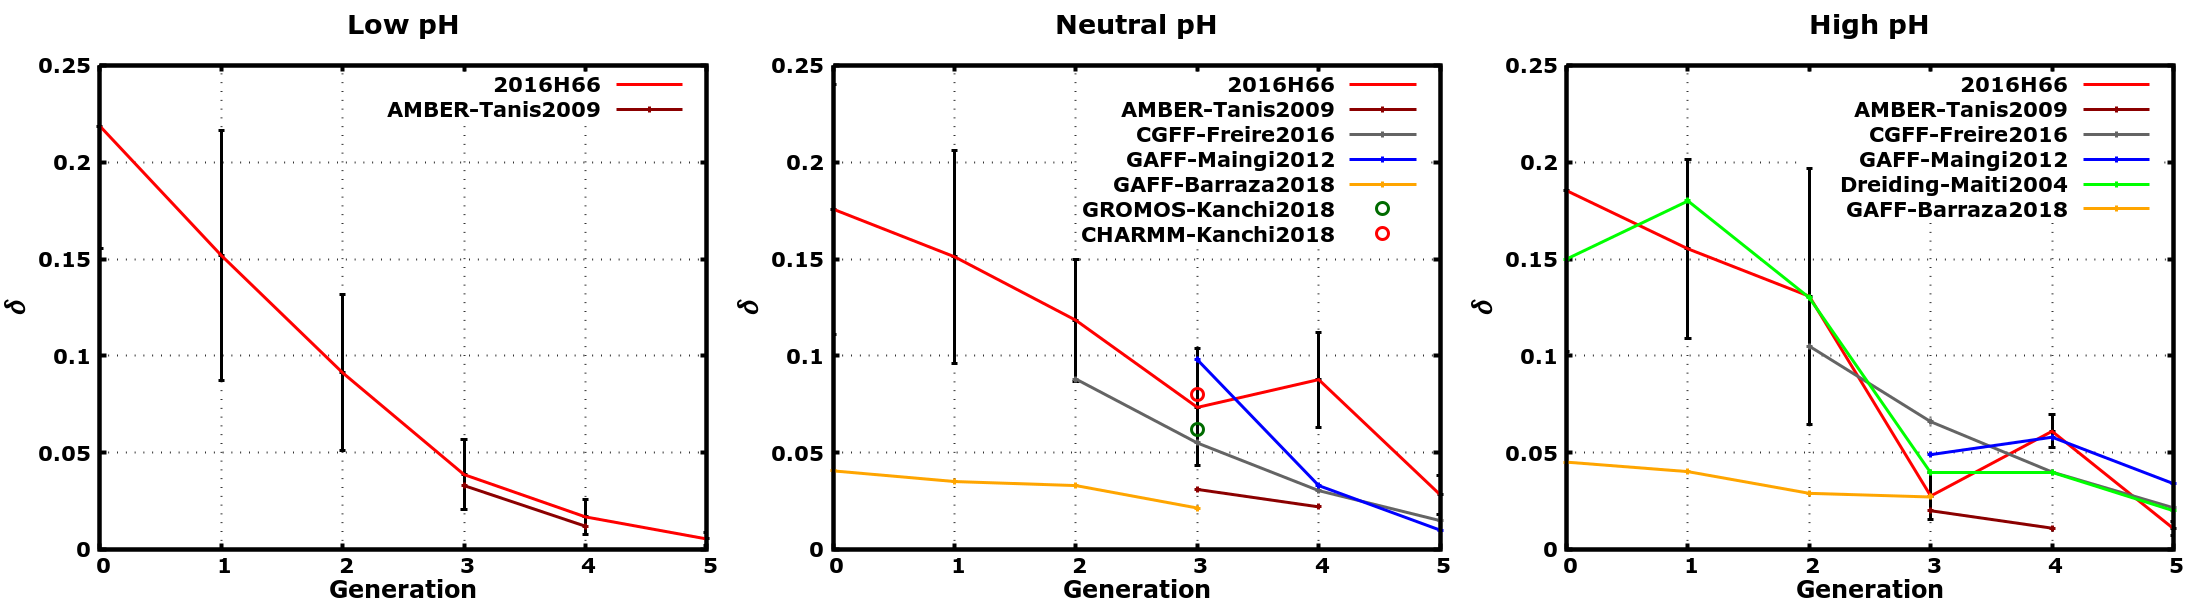
\includegraphics[width=\textwidth]{images/PAMAMAsphericity.png}
\caption{Asfericidade $\delta$ do PAMAM em função da geração. As curvas da esquerda para a direita mostram, respectivamente, os sistemas em baixo, neutro e alto pH.
Os resultados obtidos com o campo de força 2016H66\cite{Horta2016} são comparados com resultados de estudos experimentais e de simulações prévios:
Maiti2004\cite{Maiti2004}, %\cite{MA04.18},
Tanis2009\cite{Tanis2009}, %\cite{TA09.6},
Maingi2012\cite{Maingi2012}, %\cite{MA12.23},
Freire2016\cite{Freire2016}, %\cite{FR16.Y}.}
Barraza2018\cite{Barraza2018}.} %\cite{BA18.Y} and
\label{fig:PAMAMAsphericity}
\end{figure*}

\begin{table*}
\centering
    \begin{tabular}{cccccccc}
 \hline
 $GN$     & pH  & Iz/Iy &   Iz/Ix   & Asphericity\\
 \hline
 \hline 
 G0     &  \multirow{6}{*}{Acid}    &   1.2219& 1.6535& 0.2187\\
 G1     &                           &   1.5497& 1.9441& 0.1518\\
 G2     &                           &   1.1938& 1.6545& 0.0913\\
 G3     &                           &   1.2680& 1.4044& 0.0387\\
 G4     &                           &   1.3583& 1.1048& 0.0168\\
 G5     &                           &   1.0285& 1.0557& 0.0054\\
 \hline 
 G0     &  \multirow{6}{*}{Neutral} &   1.2775& 3.0340& 0.1757\\
 G1     &                           &   1.1420& 2.6886& 0.1511\\
 G2     &                           &   1.1455& 1.8338& 0.1183\\
 G3     &                           &   1.0582(1.69)& 1.1380(3.19)& 0.0734(0.098)\\
 G4     &                           &   1.1020(1.17)& 1.6704(1.93)& 0.0877(0.033)\\
 G5     &                           &   1.1473(1.13)& 1.3964(1.41)& 0.0283(0.010)\\
 \hline 
 G0     &  \multirow{6}{*}{Basic}   &   1.1418& 2.2922& 0.1853\\
 G1     &                           &   1.3091& 2.0219& 0.1552\\
 G2     &                           &   1.0367& 1.4595& 0.1308\\
 G3     &                           &   1.1530(1.38)& 1.3704(2.21)& 0.0276(0.049)\\
 G4     &                           &   1.3277(1.41)& 1.4790(2.44)& 0.0610(0.058)\\
 G5     &                           &   1.0807(1.29)& 1.2036(1.93)& 0.0108(0.034)\\
 \hline
    \end{tabular}
\caption{Tabela com os valores de razão de aspecto e asfericidades calculados com o 2016H66 para o PAMAM.
Os valores entre parênteses são dados retirados do estudo de Maingi \textit{et al}\cite{Maingi2012}.}
\label{tab:PAMAMAsfericidade}
\end{table*}

Em baixo pH, vemos um decaimento monotônico da asfericidade $\delta$ com o aumento da geração tendendo à uma esfera, ou seja, $\delta \sim 0$. 
Tanis e Karatasos\cite{Tanis2009} reportaram praticamente os mesmo valores obtidos por esse trabalho para dendrímeros de geração $3$ e $4$ em baixo pH fazendo uso do campo de força AMBER\cite{Weiner1984} e solvente explícito.

Já em pH neutro, o 2016H66 continua a mostrar um decaimento da asfericidade com a geração, mas um leve aumento ocorre na geração 4.
Valores similares foram encontrados por Maingi \textit{et al}\cite{Maingi2012} com o GAFF, Freire \textit{et al}\cite{Freire2016} com um campo de força \textit{coarse grained} e por Kanchi \textit{et al}\cite{Kanchi2018} tanto com GROMOS quanto com o CHARMM para a terceira geração.
Mas eles não apresentam o aumento mostrado pelo 2016H66\cite{Horta2016} em pH neutro.
Outros estudos como o do Barraza \textit{et al}\cite{Barraza2017} com GAFF e do Tanis e Karatasos\cite{Tanis2009} com o AMBER\cite{Weiner1984} apresentam valores muito menores do que é comumente reportado na literatura.

Quando analisamos o sistema em pH alto, os valores reportados por Maingi \textit{et al}\cite{Maingi2012} e por Maiti \textit{et al}\cite{Maiti2004} apresentam o mesmo comportamento na geração 4 que o 2016H66\cite{Horta2016} com valores numéricos significativamente próximos.
A simulação \textit{coarse grained} de Tanis \textit{et al}\cite{Tanis2009} mostra novamente um decaimento monotônico assim como em pH neutro.
E o comportamento reportado por Barraza \textit{et al}\cite{Barraza2017} e por Tanis e Karatasos\cite{Tanis2009} também continua o mesmo.

Trabalhos teóricos sugerem que a mudança da geração 3 para a 4 é caracterizada por um aumento substancial do \textit{back-folding} nos dendrímeros.
Sendo discutido até mesmo que seu padrão estrutural de \textit{dense core} poderia passar a ser melhor descrito como um \textit{dense shell} dependendo do tamanho do terminal.
Essa mudança, contudo, não ocorre no PAMAM.
Como veremos mais à frente, as curvas de distribuição radial (RDF) revelam, de fato, um aumento na quantidade de \textit{back-folding} nessa passagem.

\subsection{Estrutura}\label{PAMAMEstrutura}

As curvas de função de distribuição radial foram calculadas como descrito na Seção \ref{RDF} e os resultados estão mostrados na Figura \ref{fig:PAMAMRDF}.

\begin{figure*}[ht!]
\centering
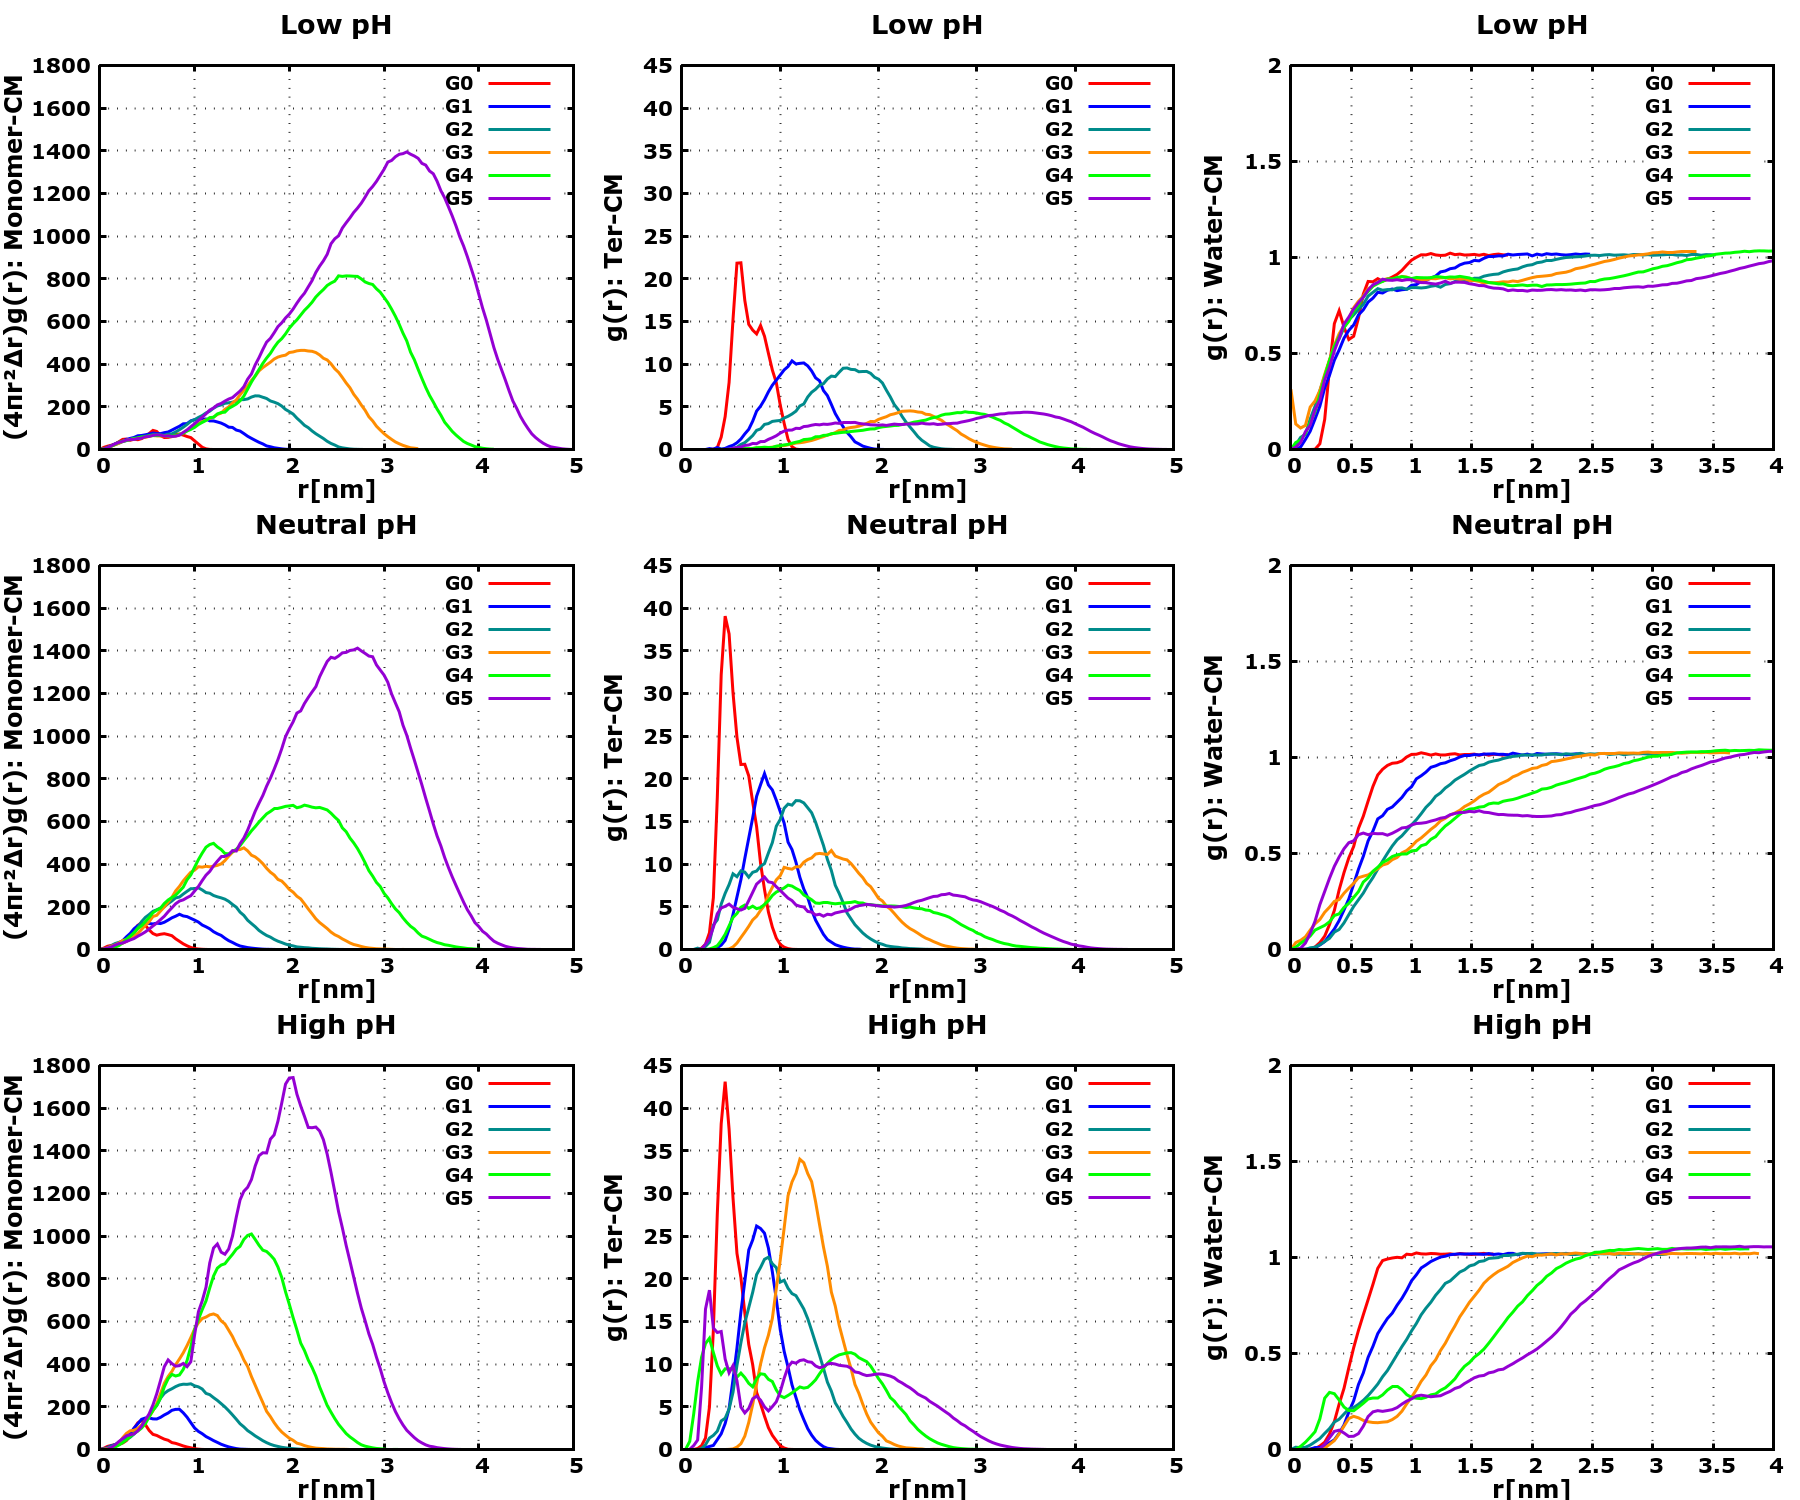
\includegraphics[width=\textwidth]{images/PAMAMRDF.png}
\caption{Função de distribuição radial (RDF) $g(r)$ para o PAMAM. As curvas da esquerda, do meio e da direita mostram, respectivamente, as RDFs do centro de massa do dendrímero em relação à todos os átomos do dendrímero, às aminas primárias terminais e às moléculas de água. E as linhas superiores, intermediárias e inferiores mostram os RDFs descritos anteriormente em condições de pH baixo, neutro e alto, respectivamente. A coluna da esquerda não foi normalizada pelo volume da camada esférica utilizada.}
\label{fig:PAMAMRDF}
\end{figure*}

A curva da esquerda mostra a função de distribuição radial sem efetuar a divisão pelo volume da casca esférica considerada no cálculo. Na prática, é o mesmo que calcular $4\pi r^2 \Delta r \times g(r)$.
Dessa forma, não podemos interpretá-la como um perfil de densidade, mas como um valor proporcional ao número absoluto de átomos contados. 
Ela mostra que o aumento da geração faz com que se forme um acúmulo de átomos na região superfícial do dendrímero.
Esse comportamento é o mesmo obtido por Lee \textit{et al}\cite{Lee2002} que pode ser visto na coluna da esqueda da Figura 11 em seu estudo.
É intuitivo pensar dessa forma devido ao fato de que cada nova geração tem o dobro de aminas terminais que a geração anterior. 
Os autores acreditam que isso foi o motivador principal para caracterizar, errôneamente, dendrímeros pelo modelo de \textit{dense shell} já que essas curvas não podem ser interpretadas como densidades.
Nela, podemos ver, também, o efeito do pH na estrutura dendrítica do PAMAM.
Conforme o pH se torna mais ácido (ou mais baixo), a distribuição se torna mais larga.
Indicando que o tamanho da molécula aumenta e que, devido à concentração de átomos na superfície, ela apresenta cavidades maiores (ou mais espaços vazios).
Isso se deve ao fato de que a protonação das aminas cria uma forte repulsão entre elas. Isso gera um afastamento que possibilita a entrada de solvente na estrutura.
Esse inchaço é amplamente reportado na literatura e foi visto ser capturado pelas simulações com o 2016H66\cite{Horta2016}.
 
A coluna do meio da Figura \ref{fig:PAMAMRDF} apresenta a função de distribuição radial das aminas primárias terminais em relação ao centro de massa do dendrímero.
Essas curvas foram normalizadas pelo volume da casca esférica. 
Por isso, podem ser chamadas de perfil de densidade das aminas terminais. 
Note que essa curva está completamente diferente das curvas reportadas por Lee \textit{et al}\cite{Lee2002} na coluna da direita da Figura 11 em seu trabalho e por Brocorens \textit{et al}\cite{Brocorens2005} na Figura 6 do seu trabalho.
A principal diferença é que ambos estão calculando funções de distribuição, e não perfis de densidade.
Como o que é calculado por Maiti \textit{et al}\cite{Maiti2004} na Figura 7 de seu trabalho e por Bellini \textit{et al}\cite{Bellini2015} na subfigura d) da Figura 2 de seu estudo, as curvas se assemelham substancialmente às reportadas nesse trabalho. 
Novamente podemos ver que para baixos pHs, o tamanho do dendrímero é maior.

Interessantemente, nesses gráficos é possível ver que mesmo com o aumento da geração, a existênciade densidade de aminas terminais ao longo de todo o volume da molécula se mantêm.
Isso se deve à formação de \textit{back-folding}, como discutido anteriormente.

O efeito do pH é de expandir a estrutura devido à repulsão eletrostática gerada pelas aminas protonadas e consequente hidratação da estrutura. Aqui vemos que a maior compactação da estrutura em pH alto é devido ao maior grau de \textit{back-folding} das aminas terminais. 
E mesmo após protonação das aminas (pH baixo) ainda é possível observar a existência de \textit{back-folding} no sistema. 
Como uma pequena massa do sistema está localizada no centro do dendrímero (devido às cavidades internas da estrutura) o fator entrópico de formar o \textit{back-folding} de partes mais externas da estrutura vence a penalidade causada pela interação de volume excludente.
Então, mesmo que energeticamente seja desfavorável, é entropicamente favorável que ocorra \textit{back-folding} em dendrímeros de gerações maiores\cite{Rathgeber2004}.

A coluna da direita mostra a distribuição de densidade radial de moléculas de água ao redor do centro de massa do dendrímero. 
Colaborando para construir as mesmas conclusões obtidas nas outras distribuições, em baixo pH a curva apresenta altos valores bem próximo ao centro do dendrímero, revelando que há uma grande quantidade de moléculas de água ao longo de todo volume da molécula.
Conforme aumentamos o pH, a estrutura vai se tornando mais compacta e a densidade de água no interior do dendrímero vai diminuido.
Esse comportamento é majoritariamente percebido para maiores gerações.
Dendrímeros de menores gerações não têm uma estrutura complexa o suficiente para permitir um alto grau de \textit{back-folding} que evitaria a entrada de água.
Esse resultado se assemelha ao reportado por Wu \textit{et al}\cite{Wu2012} para o PAMAM de geração 4 na Figura 7 de seu estudo.

\begin{figure*}[ht!]
\centering
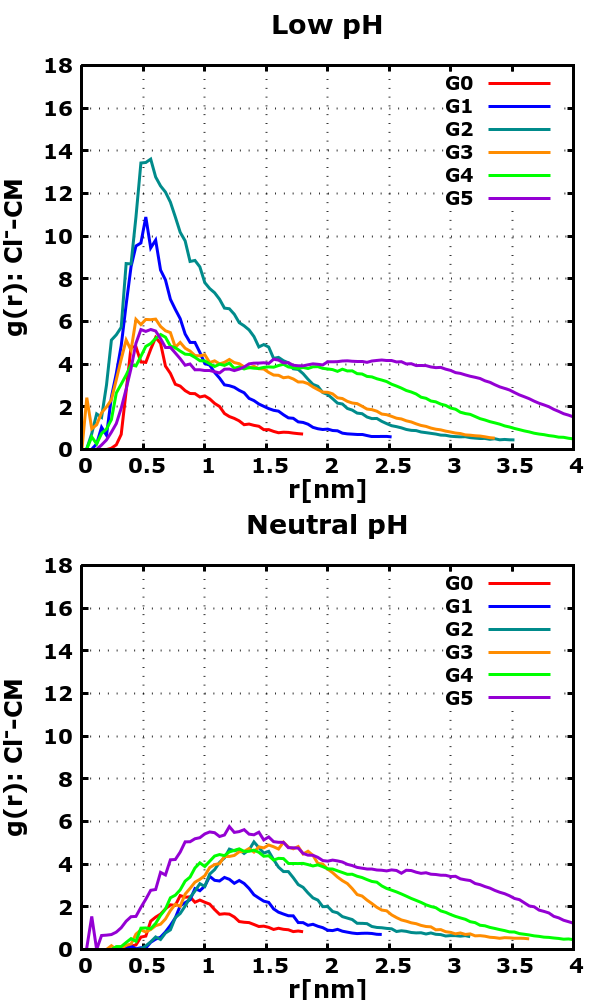
\includegraphics[scale=0.3]{images/PAMAMClRDF.png}
\caption{Função de densidade radial $g(r)$ para o PAMAM. As curvas mostram o RDF de contra-íons Cloreto em relação ao centro de massa do dendrímero para os casos onde o contra-íon está presente(pHs alto e neutro).}
\label{fig:PAMAMClRDF}
\end{figure*}

A Figura \ref{fig:PAMAMClRDF} apresenta os perfis de densidade de íons cloreto no sistema.
É interessante perceber que (imagem de cima da Figura \ref{fig:PAMAMClRDF}), a curva de distribuição dos íons apresenta um pico muito próximo do centro do dendrímero em pH baixo independentemente da geração, devido à maior concentração de carga no interior da molécula nesse pH.
Como a carga no interior da estrutura nesse pH é altamente positiva, os íon são fortemente atraídos para os sítios de carregados positivamente.
Já em pH neutro, a maior concentração de íons se dá majoritáriamente ao longo da superfície do dendrímero, onde há a concentração de cargas positivas (imagem de baixo da Figura \ref{fig:PAMAMClRDF}).

\begin{landscape}
\begin{table}[t] %PPI Rg Suplemmental info tables
\caption{
Comparação do raio de giro $R_g$ (em nm) calculado na presente dissertação para o PPI com valores disponíveis na literatura.
Os resultados estão organizados de acordo com o pH do meio (baixo, neutro e alto), número da geração $GN$ (de G1 à G6) e método utilizado no tratamento das interações de Lennard-Jones (PME: Particle-Mesh Ewald e CUT: \textit{cut-off scheme} com raio de corte de $1.2$ nm).
Como discutido na Seção \ref{ProtonacaoPPI}, somente os valores com a protonação sugerida pelo modelo de Ising\cite{VanDuijvenbode1998, Koper1997} foram considerados.
Os resultados da literatura mostrados foram tirados dos seguintes estudos:
SAXS(Prosa1997)\cite{Prosa1997},
SANS(Scherrenberg1998)\cite{Scherrenberg1998},
SANS(Topp1999)\cite{Topp1999},
COMPASS/OPLS(Wu2010)\cite{Wu2010},
GAFF(Maingi2012)\cite{Maingi2012},
GAFF(Jain2013)\cite{Jain2013}.}
\centering
\scalebox{0.8}{
\begin{tabular}{ccccccccccccc}
\hline
G$N$   & \multirow{2}{*}{pH}   &\multicolumn{2}{c}{This work}  &COMPASS/OPLS\cite{Wu2010}  &   GAFF\cite{Maingi2012}  &GAFF\cite{Jain2013}  &SANS\cite{Topp1999}  &   SAXS\cite{Prosa1997}   & SANS\cite{Scherrenberg1998}\\
PPI   &                       &       PME     &       CUT     &                       &                       &                   &                   &                       &                   \\
% PPI &                       &       PME     &       CUT     &   Wu2010              &   Maingi2012          &   Jain2013        &   Topp1999        &   Prosa1997           & Scherrenberg1998  \\
\hline
G1   &  \multirow{6}{*}{Low}    &   0.51        &   0.51        &-                      &-                      &   -               &   -               &   -                   &   -   \\
G2  &                          &   0.78        &   0.79        &-                      &-                      &   -               &   -               &   -                   &   -   \\
G3     &                          &   1.04        &   1.06        &-                      &-                      &   -               &   -               &   -                   &   -   \\
G4    &                          &   1.34        &   1.35        &-                      &-                      &   -               &   -               &   -                   &   -   \\
G5   &                          &   1.65        &   1.65        & 1.58                  &-                      &   -               &   -               &   -                   &   -   \\
G6  &                          &   1.99        &   2.00        &-                      &-                      &   -               &   -               &   -                   &   -   \\
\hline
G1    & \multirow{6}{*}{Neutral} &   0.51        &   0.51        &-                      &-                      &   -               & -                 &-                      & 0.44  \\
G2   &                          &   0.77        &   0.77        &-                      &-                      &   -               & -                 &-                      & 0.69  \\
G3  &                          &   1.04        &   1.05        &-                      &-                      &   -               & -                 & 1.13                  & 0.93  \\
G4     &                          &   1.34        &   1.32        &-                      &-                      &   -               & 1.24              & 1.33                  & 1.16  \\
G5    &                          &   1.65        &   1.64        & 1.59                  & 1.61                  &   1.577           & 1.56              & 1.43                  & 1.39  \\
G6   &                          &   1.98        &   1.97        &-                      &-                      &   -               &                   &-                      &   -   \\
\hline
G1     & \multirow{6}{*}{High}    &   0.49        &   0.49        &-                      &-                      &   -               &   -               &   -                   &   -   \\
G2    &                          &   0.74        &   0.74        &-                      &-                      &   -               &   -               &   -                   &   -   \\
G3   &                          &   0.95        &   0.94        &-                      &-                      &   -               &   -               &   -                   &   -   \\
G4  &                          &   1.07        &   1.03        &-                      &-                      &   -               &   -               &   -                   &   -   \\
G5     &                          &   1.25        &   1.31        & 1.23                  &   1.31                &   1.273           &   -               &   -                   &   -   \\
G6    &                          &   1.60        &   1.56        &-                      &-                      &   -               &   -               &   -                   &   -   \\
\hline   \end{tabular}}
\label{tab:PPIRgValidacao}
\end{table}
\end{landscape}

\section{PPI}

Os valores de raios de giro calculados estão listados na Tabela \ref{tab:PPIRgValidacao} e foram calculados de acordo com o procedimento descrito na Seção \ref{RaioDeGiro} para os sistemas PPI relatados na Seção \ref{SistemasSimulados} e na Tabela \ref{tab:sistemas}.
Em meio neutro, o grau de protonação considerado nessa discussão é o proposto pelo modelo de Ising\cite{VanDuijvenbode1998, Koper1997} como discutido na Seção \ref{ProtonacaoPPI}.

\subsection{Tamanho}\label{PPITamanho}

\begin{figure*}[ht!]
\centering
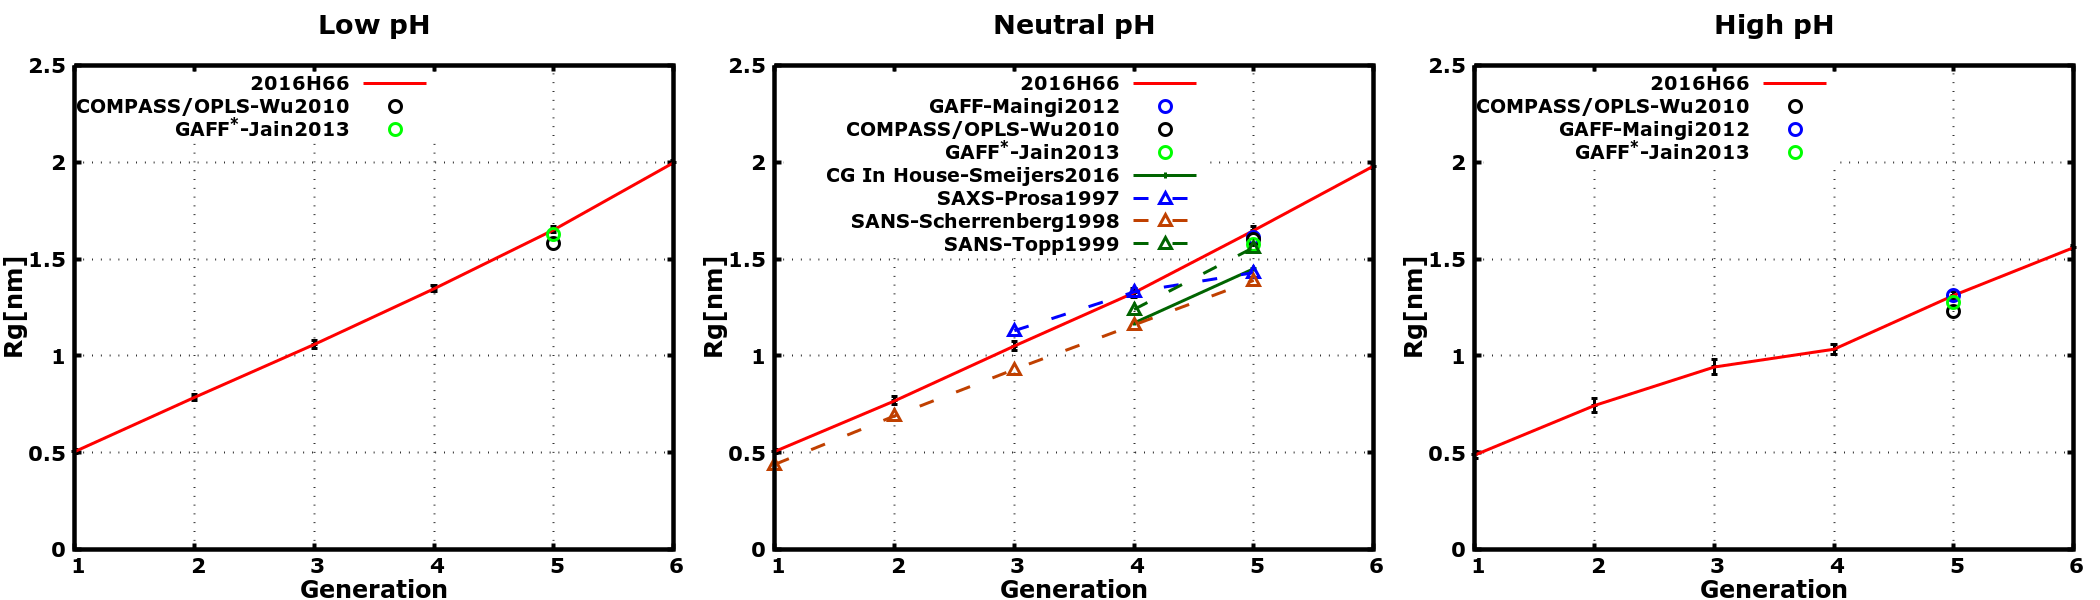
\includegraphics[width=\textwidth]{images/PPIRg.png}
\caption{Raio de giro ($R_g$) em função da geração em meios de pH baixo (curva da esquerda), neutro (curva do meio) e alto (curva da direita).
Os resultados obtidos com o campo de força 2016H66\cite{Horta2016} são comparados com resultados de estudos experimentais e de simulações prévios:
Prosa1997\cite{Prosa1997}, %\cite{PR97.2},
Scherrenberg1998\cite{Scherrenberg1998}, %\cite{SC98.Y},
Topp1999\cite{Topp1999}, %\cite{TO99.Y},
Wu2010\cite{Wu2010}, %\cite{WU10.5},
Maingi2012\cite{Maingi2012}, %\cite{MA12.23},
Jain2013\cite{Jain2013}, %\cite{JA13.4}}
Smeijers2016\cite{Smeijers2016}.} %\cite{SM16.Y}
\label{fig:PPIRg}
\end{figure*}

Um problema encontrado na validação do PPI, é a falta de dados reportados na literatura para tal. Muitos dos estudos efetuados com o PPI são fortemente focados em aplicações.
Por isso, não foram encontrados estudos de simulação sistemáticos onde a influência do raio de giro foi levado em conta.
Principalmente em pHs ácido e básico, onde não haviam dados experimentais disponíveis.

Em baixo pH, na Figura \ref{fig:PPIRg}, os resultados do 2016H66\cite{Horta2016} está em excelente acordo com os trabalhos de Wu\cite{Wu2010}, que utiliza um campo de força composto por uma mistura de parâmetros do Compass\cite{Sun1998} e do OPLS-AA\cite{Jorgensen1996}, e de Jain \textit{et al}\cite{Jain2013} que aplica o GAFF\cite{Wang2004} em um PPI com núcleo de EDA, ao inves de DAB como feito nesse trabalho.
Contudo, os resultados são bem próximos mostrando que um núcleo diferente mas com mesma valência não influencia fortemente o raio de giro da molécula.

Já em pH neutro, há uma maior quantidade de dados, inclusive experimentais, para comparação.
Nesse meio, os resultados para a geração 5 de Wu\cite{Wu2010} e de Jain \textit{et al}\cite{Jain2013} continuam a ter um excelente acordo com o 2016H66\cite{Horta2016}. 
Os resultados obtidos com o 2016H66\cite{Horta2016} também estão em bom acordo com o estudo de Maingi \textit{et al}\cite{Maingi2012}.
Para a mesma geração, dados de SANS reportados por Topp \textit{et al}\cite{Topp1999} mostram relativo acordo com os trabalhos de simulação apresentados.
Esse trabalho com SANS mostra um raio de giro em torno de $0.1$ nm menor que o obtido pelo 2016H66\cite{Horta2016}.
Essa diferença se mantém quando em geração 4.
Outro conjunto de valores reportados por SANS estão disponíveis no estudo de Scherrenberg \textit{et al}\cite{Scherrenberg1998}.
Considerando esse conjunto, os resultados obtidos com o 2016H66\cite{Horta2016} continuam a consistentemente superestimar os dados experimentais, mas não mais com uma diferença constante.
Pode-se ver que a divergência entre os dados aumenta com o aumento da geração do PPI.
Curiosamente, os dados de SAXS reportados por Prosa \textit{et al}\cite{Prosa1997} novamente apresentam um perfil fortemente discordante do padrão aproximadamente linear visto nos outros conjuntos apresentados, assim como para seu estudo no PAMAM.
%%%%%%%%%%%%%%%%%%% SANS BRUNO %%%%%%%%%%%%%%%%%%%
Mesmo com todos os problemas reportados anteriormente para dados de SANS\cite{Porcar2008} na Seção \ref{PAMAMTamanho} (principalmente a invariância com o pH) que sugeriam que estudos de SAXS\cite{Rathgeber2002} seriam mais indicados para o estudo de dendrímeros, o cenário para o PPI ainda é inconclusivo.
Nada pode ser afirmado uma vez que não existem dados de estudos experimentais em diferentes pHs para o PPI.

Em pH básico (ou alto), temos o mesmo cenário que em ácido.
Os valores disponíveis por simulação utilizando tanto COMPASS/OPLS-AA\cite{Wu2010} quanto GAFF com núcleos de EDA\cite{Jain2013} ou de DAB\cite{Maingi2012} estão de acordo ao menos para a geração 5.

\begin{figure*}[ht!]
\centering
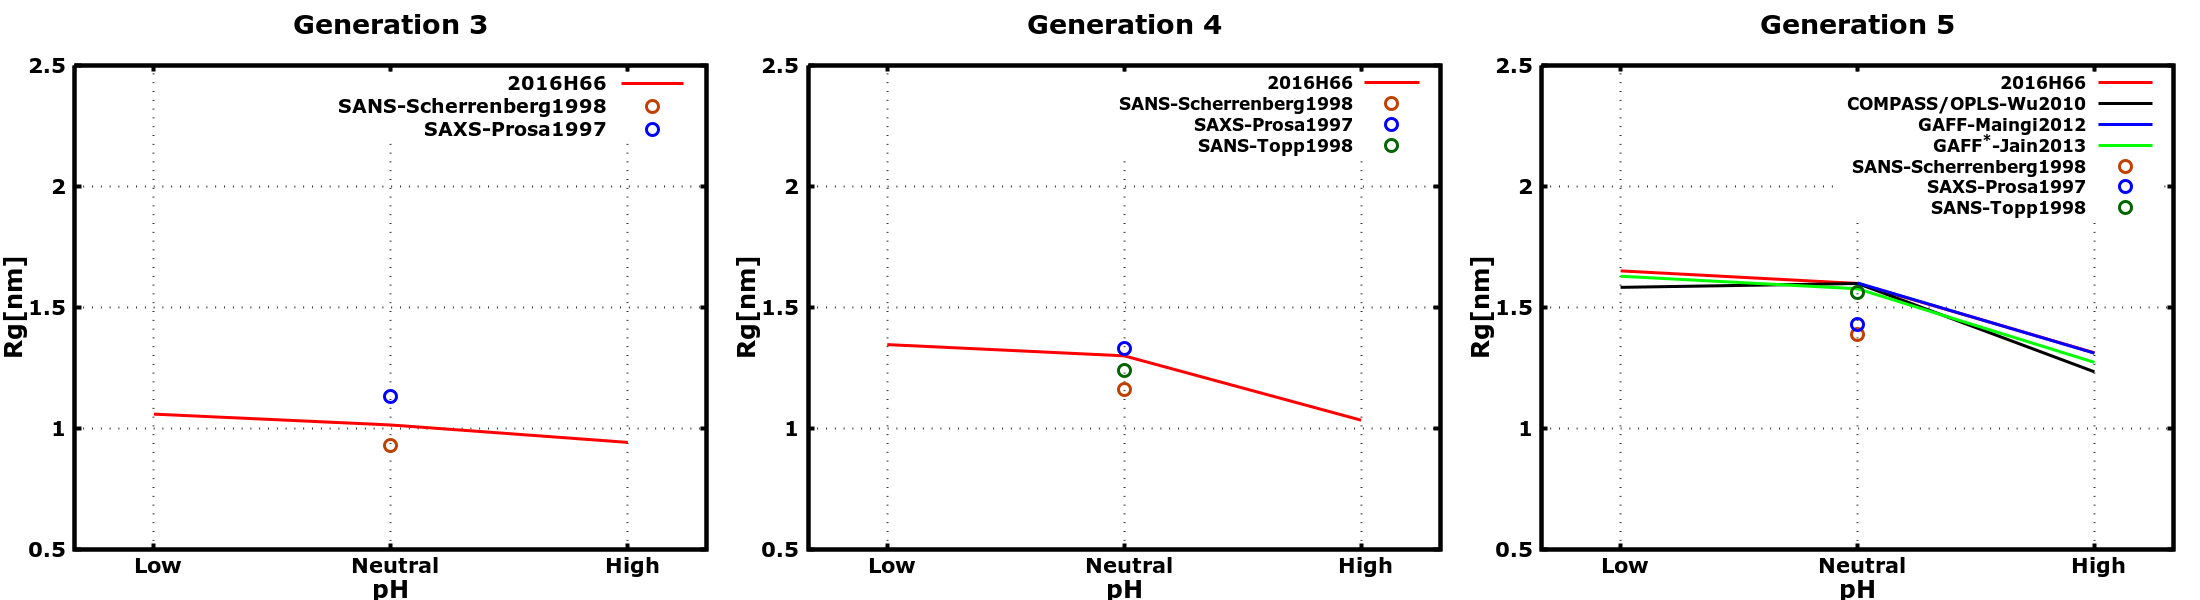
\includegraphics[width=\textwidth]{images/PPIgyrateGpH.png}
\caption{Raio de giro ($R_g$) em função do pH para o PPI de geração 3 (curva da esquerda), 4 (curva do meio) e 5 (curva da direita).
Os resultados obtidos com o campo de força 2016H66\cite{Horta2016} são comparados com resultados de estudos experimentais e de simulações prévios:
Prosa1997\cite{Prosa1997}, %\cite{PR97.2},
Scherrenberg1998\cite{Scherrenberg1998}, %\cite{SC98.Y},
Topp1999\cite{Topp1999}, %\cite{TO99.Y},
Wu2010\cite{Wu2010}, %\cite{WU10.5},
Maingi2012\cite{Maingi2012}, %\cite{MA12.23},
Jain2013\cite{Jain2013}, %\cite{JA13.4}}
Smeijers2016\cite{Smeijers2016}.} %\cite{SM16.Y} and
\label{fig:PPIRgpH}
\end{figure*}

Na Figura \ref{fig:PPIRgpH}, mostramos a mesma análise feita para o PAMAM na Figura \ref{fig:PAMAMRgpH}.
Nela podemos ver com mais detalhes principalmente o sistema em pH neutro, já que em pH ácido e básico os trabalhos de simulação estão em excelente acordo com o 2016H66\cite{Horta2016}.
Vale notar que os pontos em geração 5 (imagem da direita na Figura \ref{fig:PPIRgpH}) para o 2016H66\cite{Horta2016} e para GAFF\cite{Mayo1990} reportados por Maingi \textit{et al}\cite{Maingi2012} se sobrepõem.
Consultando a Tabela \ref{tab:PPIRgValidacao}, vemos que em pH neutro o 2016H66\cite{Horta2016} e o GAFF\cite{Maingi2012} resultam em $1.599$ nm e $1.601$ nm e, em pH alto, $1.312$ nm e $1.311$ nm, respectivamente.

É interessante notar que praticamente todo inchaço visto no PPI acontece quando as aminas primárias (terminais) são protonadas.
A protonação das aminas terciárias (intermediárias) causa um efeito muito menor no raio de giro da molécula.
A Figura \ref{fig:PPIRgpH} e o Tabela \ref{tab:PPIRgValidacao} mostra que, para a geração 4, na passagem do pH alto para o neutro, ou seja, quando as aminas terminais são protonadas, o raio de giro vai de $1.03$ nm para $1.32$ nm.
Um inchaço relativo de, aproximadamente, $22\%$.
Enquanto quando varia o pH de neutro para baixo, têm-se um inchaço de apenas 2\%, mesmo que as aminas terciárias estejam numa região mais interna do dendrímero. O raio de giro em pH baixo é de $1.35$ nm.


\subsection{Forma}\label{PPIForma}

Os fatores de forma e asfericidades foram calculados de acordo com o descrito na Seção \ref{Asfericidade} para os sistemas reportados na Seção \ref{SistemasSimulados}.
Os valores das propriedades obtidas estão disponíveis na Tabela \ref{tab:PPIAsfericidade}.
Sob as suposições discutidas na Seção \ref{EfeitoDoSetup}, somente as propriedades obtidas com o esquema de avaliação das interações de Lennard-Jones sendo o \textit{cut-off} e considerando o estado de protonação proposto pelo modelo de Ising\cite{VanDuijvenbode1998, Koper1997} para o pH neutro são exibidos.

\begin{figure*}[ht!]
\centering
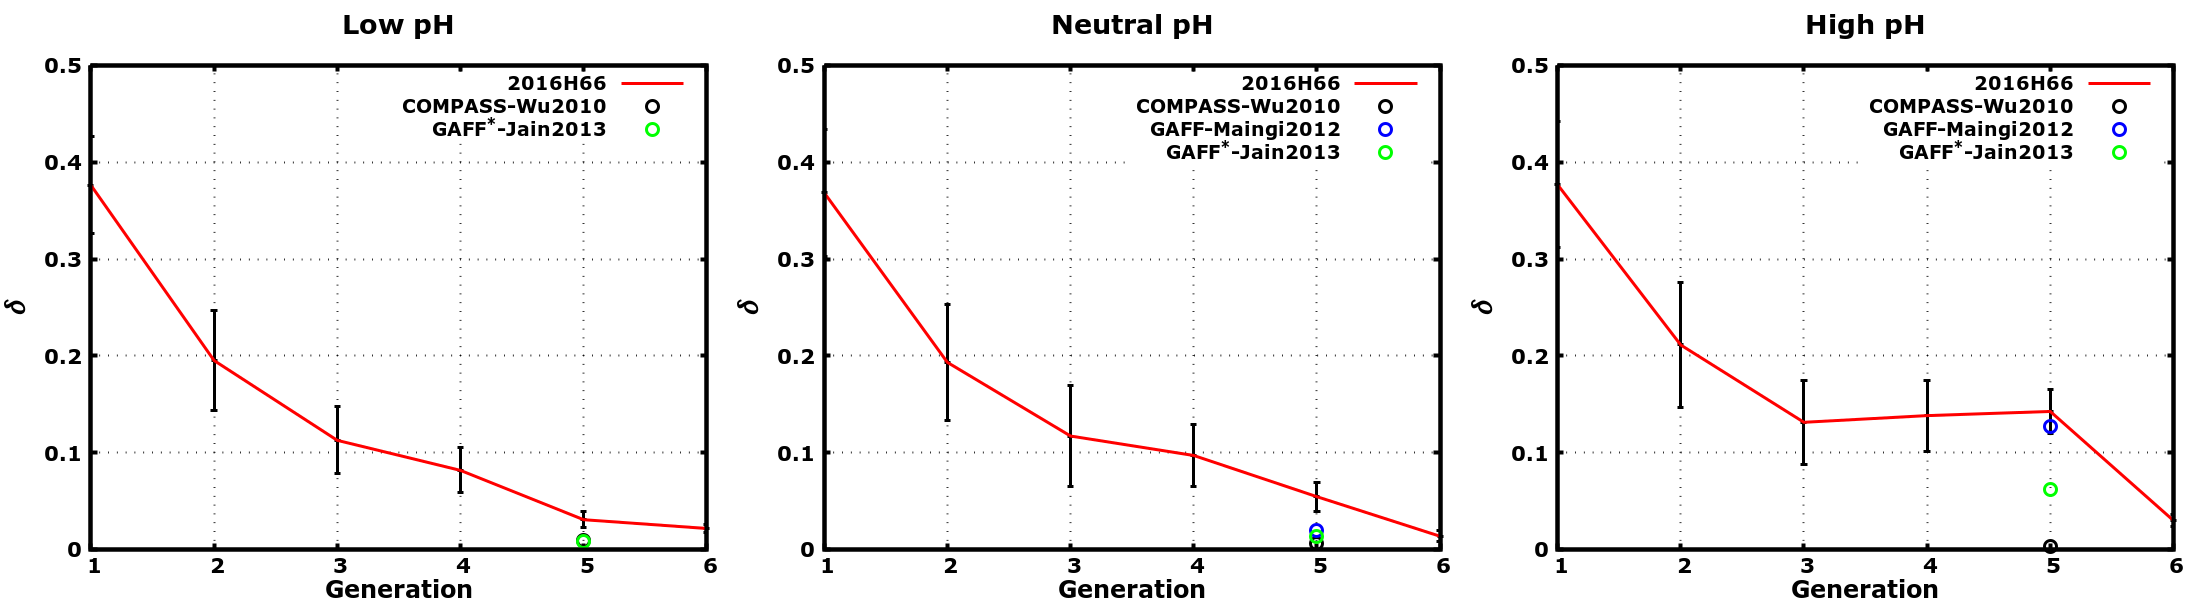
\includegraphics[width=\textwidth]{images/PPIAsphericity.png}
\caption{Asfericidade $\delta$ do PPI em função da geração. As curvas da esqueda para a direita mostram os sistemas em baixo, neutro e alto pH, respectivamente.
Os resultados obtidos com o campo de força 2016H66\cite{Horta2016} são comparados com resultados de estudos experimentais e de simulações prévios:
Wu2010\cite{Wu2010}, %\cite{WU10.5}, 
Maingi2012\cite{Maingi2012}, %\cite{MA12.23}, 
Jain2013\cite{Jain2013}.} %\cite{JA13.4}}
\label{fig:PPIAsphericity}
\end{figure*}

\begin{table*}[ht!] %The moments of inertia were calculated, but I don't know if they are really expressives
\centering
    \begin{tabular}{ccccccccccc}
 \hline
 $GN$   & pH  &   Iz/Iy   &   Iz/Ix   & Asphericity   \\
 \hline
 \hline%WU10.Y
 G1     &  \multirow{6}{*}{Acid}    &   1.2555&4.3832&0.3762\\
 G2     &                           &   1.4106&2.2934&0.1951\\
 G3     &                           &   1.3554&1.8071&0.1127\\
 G4     &                           &   1.2671&1.5132&0.0817\\
 G5     &                           &   1.1565&1.3290&0.0308\\
 G6     &                           &   1.1865&1.2995&0.0217\\
 \hline
 G1     &  \multirow{6}{*}{Neutral} &   1.2882&2.8412&0.3685\\
 G2     &                           &   1.3852&2.1706&0.1932\\
 G3     &                           &   1.0299&1.7626&0.1172\\
 G4     &                           &   1.0965&1.7413&0.0971\\
 G5     &                           &   1.1552(1.35)&1.3358(1.58)&0.0546(0.020)\\
 G6     &                           &   1.0670&1.2045&0.0136\\
 \hline
 G1     &  \multirow{6}{*}{Basic}   &   1.2443&3.8218&0.3768\\
 G2     &                           &   1.1224&2.7673&0.2112\\
 G3     &                           &   1.2986&2.3075&0.1314\\
 G4     &                           &   1.1288&2.0480&0.1383\\
 G5     &                           &   1.2782(1.56)&2.0844(4.36)&0.1426(0.127)\\
 G6     &                           &   1.2657&1.3948&0.0299\\
 \hline
    \end{tabular}
\caption{Tabela com os valores de razão de aspecto e asfericidade calculados com o 2016H66 para o PPI. Os valores entre parênteses são dados retirados do estudo de Maingi \textit{et al} \cite{Maingi2012}.}
\label{tab:PPIAsfericidade}
\end{table*}

Como a asfericidade não é uma propriedade quantitativamente mensurável a partir de técnicas experimentais, a escassez de trabalhos disponíveis na literatura dificultou a validação ainda mais nessa etapa.

Em pH baixo, os valores de asfericidade reportados na literatura por Wu \textit{et al}\cite{Wu2012} quanto por Jain \textit{et al}\cite{Jain2013} estão em acordo com os resultados do 2016H66\cite{Horta2016}.

Porém, em pH neutro é possível notar uma distanciação considerável entre os modelos.
Tanto para os citados anteriormente quanto para os dados de Maingi \textit{et al}\cite{Maingi2012}, onde o 2016H66\cite{Horta2016} apresenta um acordo um pouco melhor com esse último.

No pH alto, os resultados de outros estudos de simulação divergem fortemente.
Os resultados de COMPASS/OPLS-AA de Wu \textit{et al}\cite{Wu2010} seguem com uma estrutura fortemente esférica (assim como em outros pHs) enquanto os de Jain \textit{et al}\cite{Jain2013} se tornam menos esféricos, como o esperado.
Dentre os trabalhos disponíveis, o 2016H66\cite{Horta2016} tem um melhor acordo com os dados apresentados por Maingi \textit{et al}\cite{Maingi2012} utilizando o campo de força GAFF\cite{Wang2004}.


\subsection{Estrutura}\label{PPIEstrutura}

\begin{figure}[ht!]
\centering
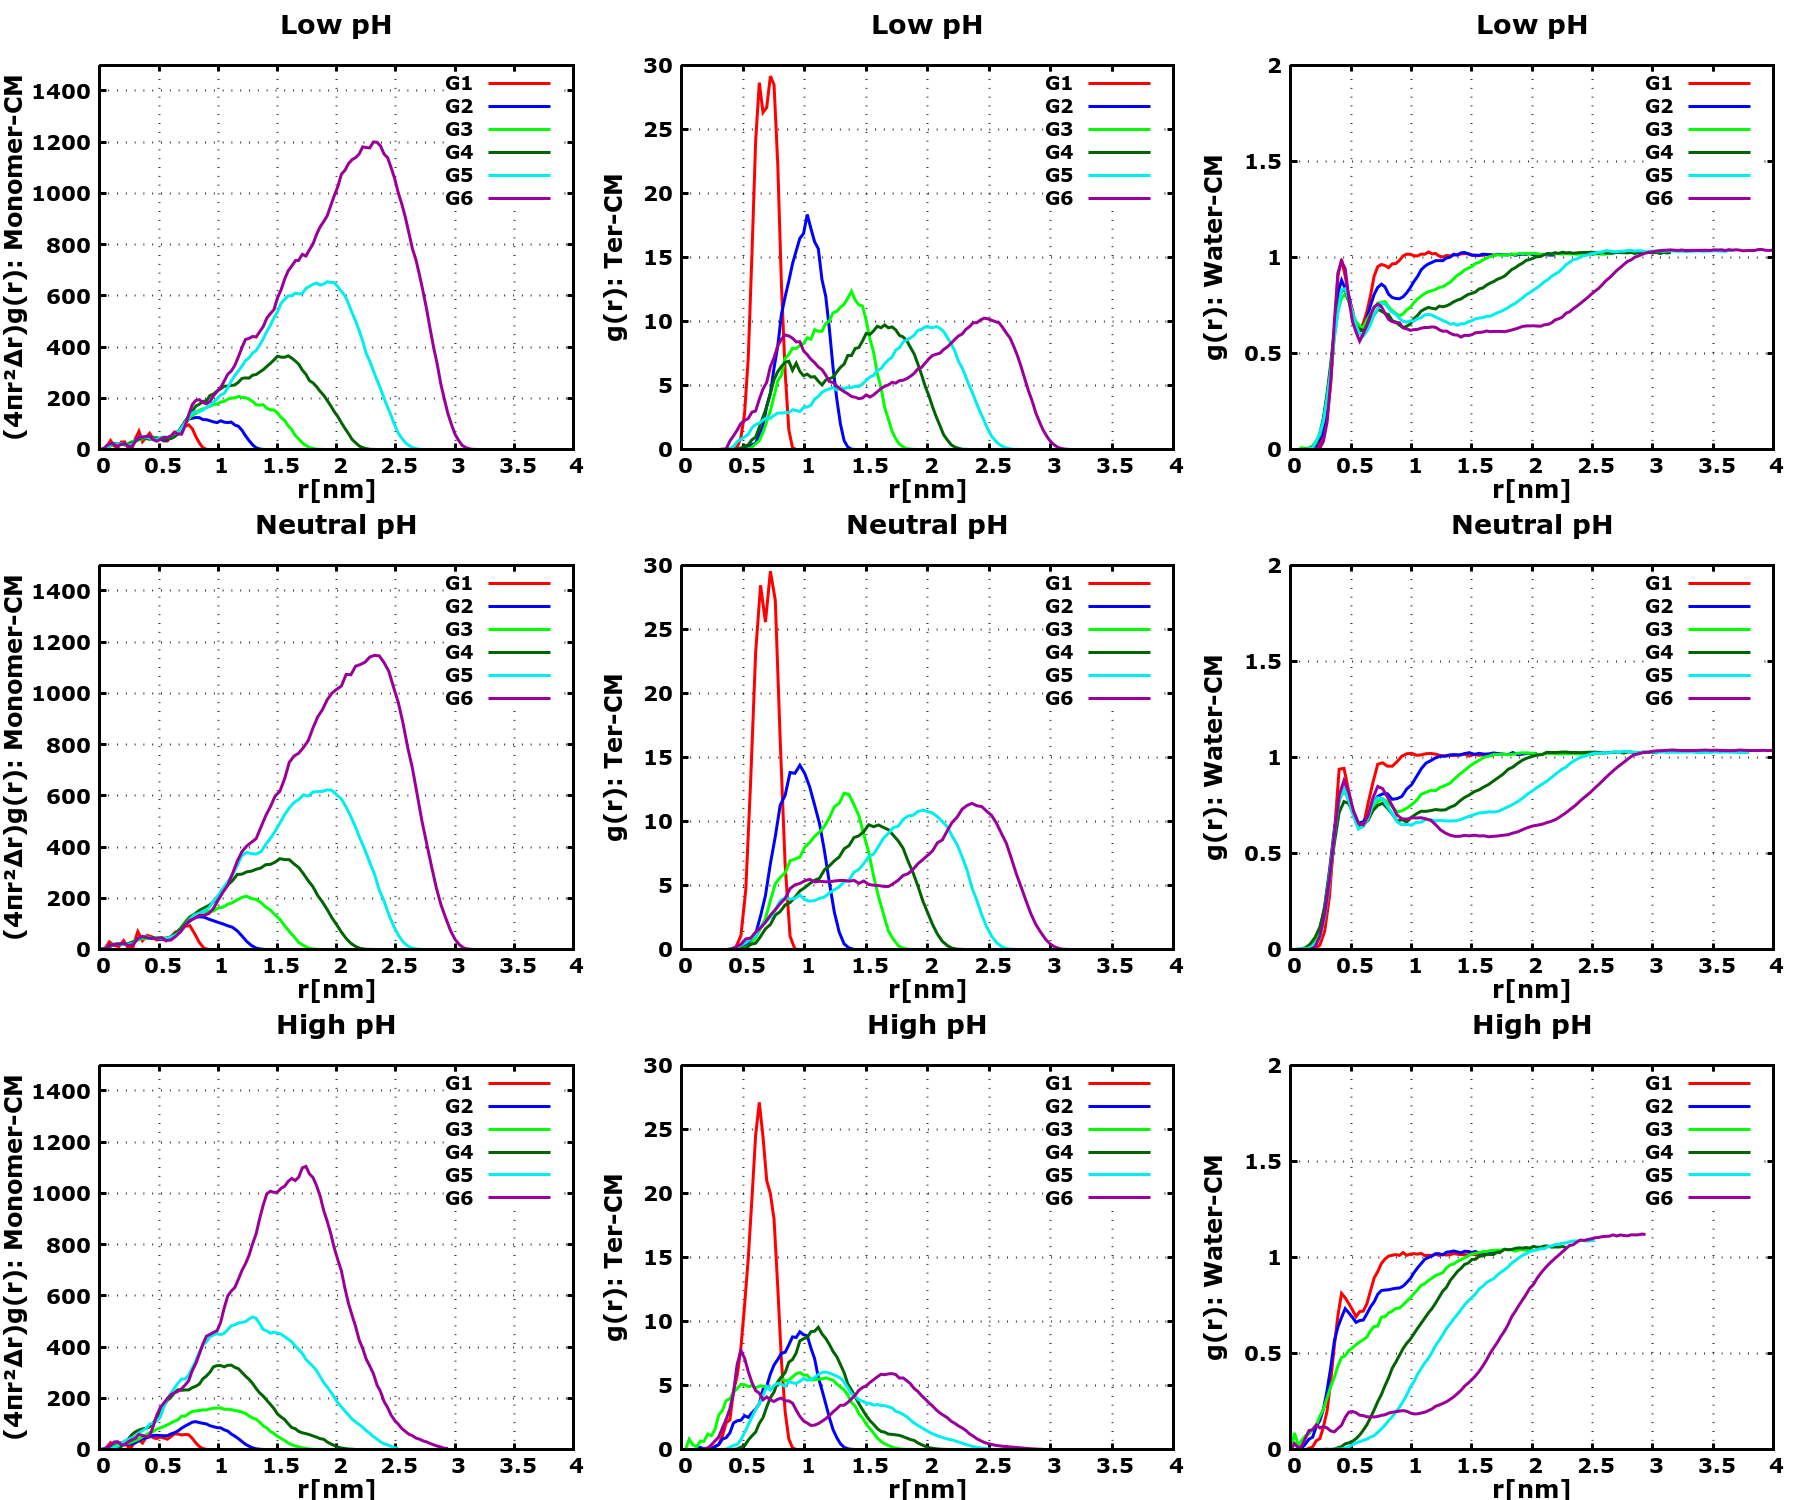
\includegraphics[width=\textwidth]{images/PPIRDF.png}
\caption{Função de distribuição radial (RDF) $g(r)$ para o PAMAM. As curvas da esquerda, do meio e da direita mostram, respectivamente, as RDFs do centro de massa do dendrímero em relação à todos os átomos do dendrímero, às aminas primárias terminais e às moléculas de água. E as linhas superiores, intermediárias e inferiores mostram os RDFs descritos anteriormente em condições de pH baixo, neutro e alto, respectivamente. A coluna da esquerda não foi normalizada pelo volume da camada esférica utilizada.}
\label{fig:PPIRDF}
\end{figure}

A função de distribuição radial foi calculada como descrito na Seção \ref{RDF} e os resultados estão exibidos na Figura \ref{fig:PPIRDF}.
As curvas refletem, no geral, um comportamento bastante parecidos com os do PAMAM.

Na coluna da esquerda, as curvas de distribuição radial de átomos ao redor do centro de massa do dendrímero (sem normalização pelo volume da camada esférica) mostram o inchaço do dendrímero com o abaixamento do pH.
Contudo, esse inchaço é menos abrupto que o observado anteriormente para o PAMAM na Seção \ref{PAMAMEstrutura}.
Os blocos de construção utilizados na montagem do PPI são significativamente menores que os componentes do PAMAM. 
Dessa forma, o incremento de tamanho no PPI com o aumento da geração é bem menor comparado ao PAMAM.
O que podemos perceber pela comparação entre os raios de giro de gerações análogas.
Além disso, de forma geral, o efeito repulsivo e posterior entrada de solvente causada pela protonação de aminas internas no PPI é menos intenso que no PAMAM.

A coluna do meio mostra a densidade radial de aminas terminais em relação ao centro de massa da molécula.
O padrão de alto grau de \textit{back-folding} em alto pH e um menor grau em baixo pH se mantém para o PPI.
Porém, diferentemente do PAMAM, para essa molécula um máximo mais acentuado de densidade de aminas terminais se mantém mais próximo ao centro do dendrímero em pH ácido.
%Como o PPI é um dendrímero menor que o PAMAM, ele apresenta uma menor complexidade em sua estrutura. o que torna possível que as aminas primárias acessem com maior facilidade seu interior.
Mesmo após a protonação da molécula.

A coluna da direita mostra a densidade radial de água no interior da estrutura do dendrímero.
Diferentemente do PAMAM, vemos que em pH neutro, o acesso de solvente no interior da estrutura é maior no PPI.
%Isso se deve à menor complexidade molecular que facilita a difusão de moléculas de água para seu interior.
%Devido à isso, a hidratação em meio neutro e ácido são bastante semelhantes.
Mas em pH básico, o alto grau de \textit{back-folding} continua a ser o efeito dominante, fazendo com que a estrutura mais compacta inviabilise a entrada de solvente.
Este resultado foi reportado, também, por Wu \textit{et al}\cite{Wu2010} na subfigura c da Figura 5 de seu artigo.

As curvas de densidade radiais de cloretos ao redor do centro de massa do dendrímero para o PPI, não difere muito para a do PAMAM. Como pode ser visto na Figura \ref{fig:PPIClRDF}.

\begin{figure}[ht!]
\centering
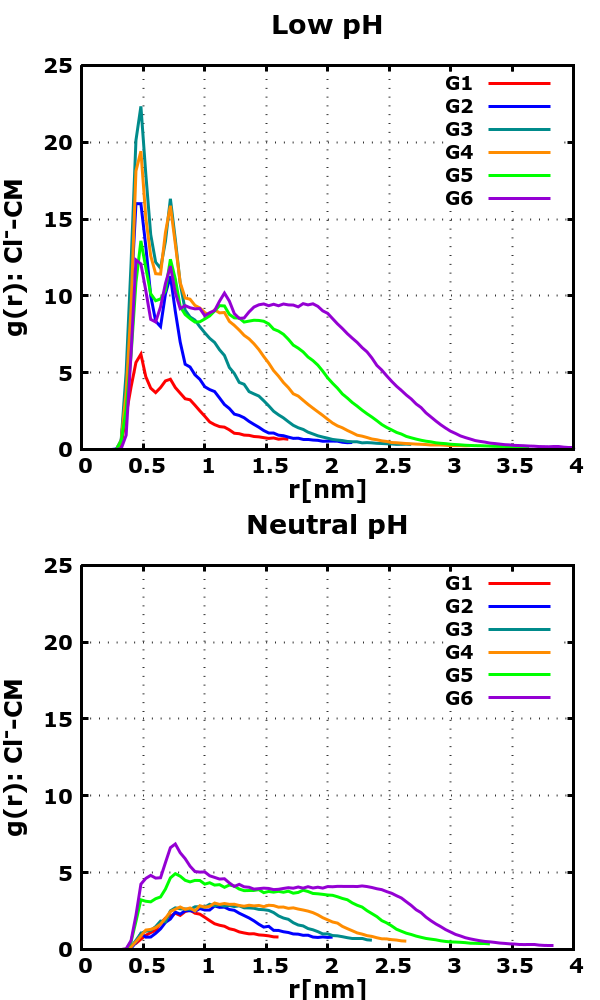
\includegraphics[scale=0.3]{images/PPIClRDF.png}
\caption{Função de distribuição radial g(r) para o PPI. As curvas mostram o RDF de contra-íons cloreto em relação ao centro de massa do dendrímero para os casos onde o contra-íon está presente(pHs alto e neutro).}
\label{fig:PPIClRDF}
\end{figure}

%Como foi discutido anteriormente nessa seção, a difusão de moléculas para o interior do PPI é mais fácil que no PAMAM devido à sua menor complexidade estrutural. 
%Contudo, isso não causa um grande impacto na distribuição de contra-íons.
%A similaridade entre as curvas de distribuições sugere que como átomos de Cloreto são bem menores que moléculas de água, a sua difusão para o interior das estruturas é mais fácil.

\pagebreak
